\documentclass[1p]{elsarticle_modified}
%\bibliographystyle{elsarticle-num}

%\usepackage[colorlinks]{hyperref}
%\usepackage{abbrmath_seonhwa} %\Abb, \Ascr, \Acal ,\Abf, \Afrak
\usepackage{amsfonts}
\usepackage{amssymb}
\usepackage{amsmath}
\usepackage{amsthm}
\usepackage{scalefnt}
\usepackage{amsbsy}
\usepackage{kotex}
\usepackage{caption}
\usepackage{subfig}
\usepackage{color}
\usepackage{graphicx}
\usepackage{xcolor} %% white, black, red, green, blue, cyan, magenta, yellow
\usepackage{float}
\usepackage{setspace}
\usepackage{hyperref}

\usepackage{tikz}
\usetikzlibrary{arrows}

\usepackage{multirow}
\usepackage{array} % fixed length table
\usepackage{hhline}

%%%%%%%%%%%%%%%%%%%%%
\makeatletter
\renewcommand*\env@matrix[1][\arraystretch]{%
	\edef\arraystretch{#1}%
	\hskip -\arraycolsep
	\let\@ifnextchar\new@ifnextchar
	\array{*\c@MaxMatrixCols c}}
\makeatother %https://tex.stackexchange.com/questions/14071/how-can-i-increase-the-line-spacing-in-a-matrix
%%%%%%%%%%%%%%%

\usepackage[normalem]{ulem}

\newcommand{\msout}[1]{\ifmmode\text{\sout{\ensuremath{#1}}}\else\sout{#1}\fi}
%SOURCE: \msout is \stkout macro in https://tex.stackexchange.com/questions/20609/strikeout-in-math-mode

\newcommand{\cancel}[1]{
	\ifmmode
	{\color{red}\msout{#1}}
	\else
	{\color{red}\sout{#1}}
	\fi
}

\newcommand{\add}[1]{
	{\color{blue}\uwave{#1}}
}

\newcommand{\replace}[2]{
	\ifmmode
	{\color{red}\msout{#1}}{\color{blue}\uwave{#2}}
	\else
	{\color{red}\sout{#1}}{\color{blue}\uwave{#2}}
	\fi
}

\newcommand{\Sol}{\mathcal{S}} %segment
\newcommand{\D}{D} %diagram
\newcommand{\A}{\mathcal{A}} %arc


%%%%%%%%%%%%%%%%%%%%%%%%%%%%%5 test

\def\sl{\operatorname{\textup{SL}}(2,\Cbb)}
\def\psl{\operatorname{\textup{PSL}}(2,\Cbb)}
\def\quan{\mkern 1mu \triangleright \mkern 1mu}

\theoremstyle{definition}
\newtheorem{thm}{Theorem}[section]
\newtheorem{prop}[thm]{Proposition}
\newtheorem{lem}[thm]{Lemma}
\newtheorem{ques}[thm]{Question}
\newtheorem{cor}[thm]{Corollary}
\newtheorem{defn}[thm]{Definition}
\newtheorem{exam}[thm]{Example}
\newtheorem{rmk}[thm]{Remark}
\newtheorem{alg}[thm]{Algorithm}

\newcommand{\I}{\sqrt{-1}}
\begin{document}

%\begin{frontmatter}
%
%\title{Boundary parabolic representations of knots up to 8 crossings}
%
%%% Group authors per affiliation:
%\author{Yunhi Cho} 
%\address{Department of Mathematics, University of Seoul, Seoul, Korea}
%\ead{yhcho@uos.ac.kr}
%
%
%\author{Seonhwa Kim} %\fnref{s_kim}}
%\address{Center for Geometry and Physics, Institute for Basic Science, Pohang, 37673, Korea}
%\ead{ryeona17@ibs.re.kr}
%
%\author{Hyuk Kim}
%\address{Department of Mathematical Sciences, Seoul National University, Seoul 08826, Korea}
%\ead{hyukkim@snu.ac.kr}
%
%\author{Seokbeom Yoon}
%\address{Department of Mathematical Sciences, Seoul National University, Seoul, 08826,  Korea}
%\ead{sbyoon15@snu.ac.kr}
%
%\begin{abstract}
%We find all boundary parabolic representation of knots up to 8 crossings.
%
%\end{abstract}
%\begin{keyword}
%    \MSC[2010] 57M25 
%\end{keyword}
%
%\end{frontmatter}

%\linenumbers
%\tableofcontents
%
\newcommand\colored[1]{\textcolor{white}{\rule[-0.35ex]{0.8em}{1.4ex}}\kern-0.8em\color{red} #1}%
%\newcommand\colored[1]{\textcolor{white}{ #1}\kern-2.17ex	\textcolor{white}{ #1}\kern-1.81ex	\textcolor{white}{ #1}\kern-2.15ex\color{red}#1	}

{\Large $\underline{11a_{344}~(K11a_{344})}$}

\setlength{\tabcolsep}{10pt}
\renewcommand{\arraystretch}{1.6}
\vspace{1cm}\begin{tabular}{m{100pt}>{\centering\arraybackslash}m{274pt}}
\multirow{5}{120pt}{
	\centering
	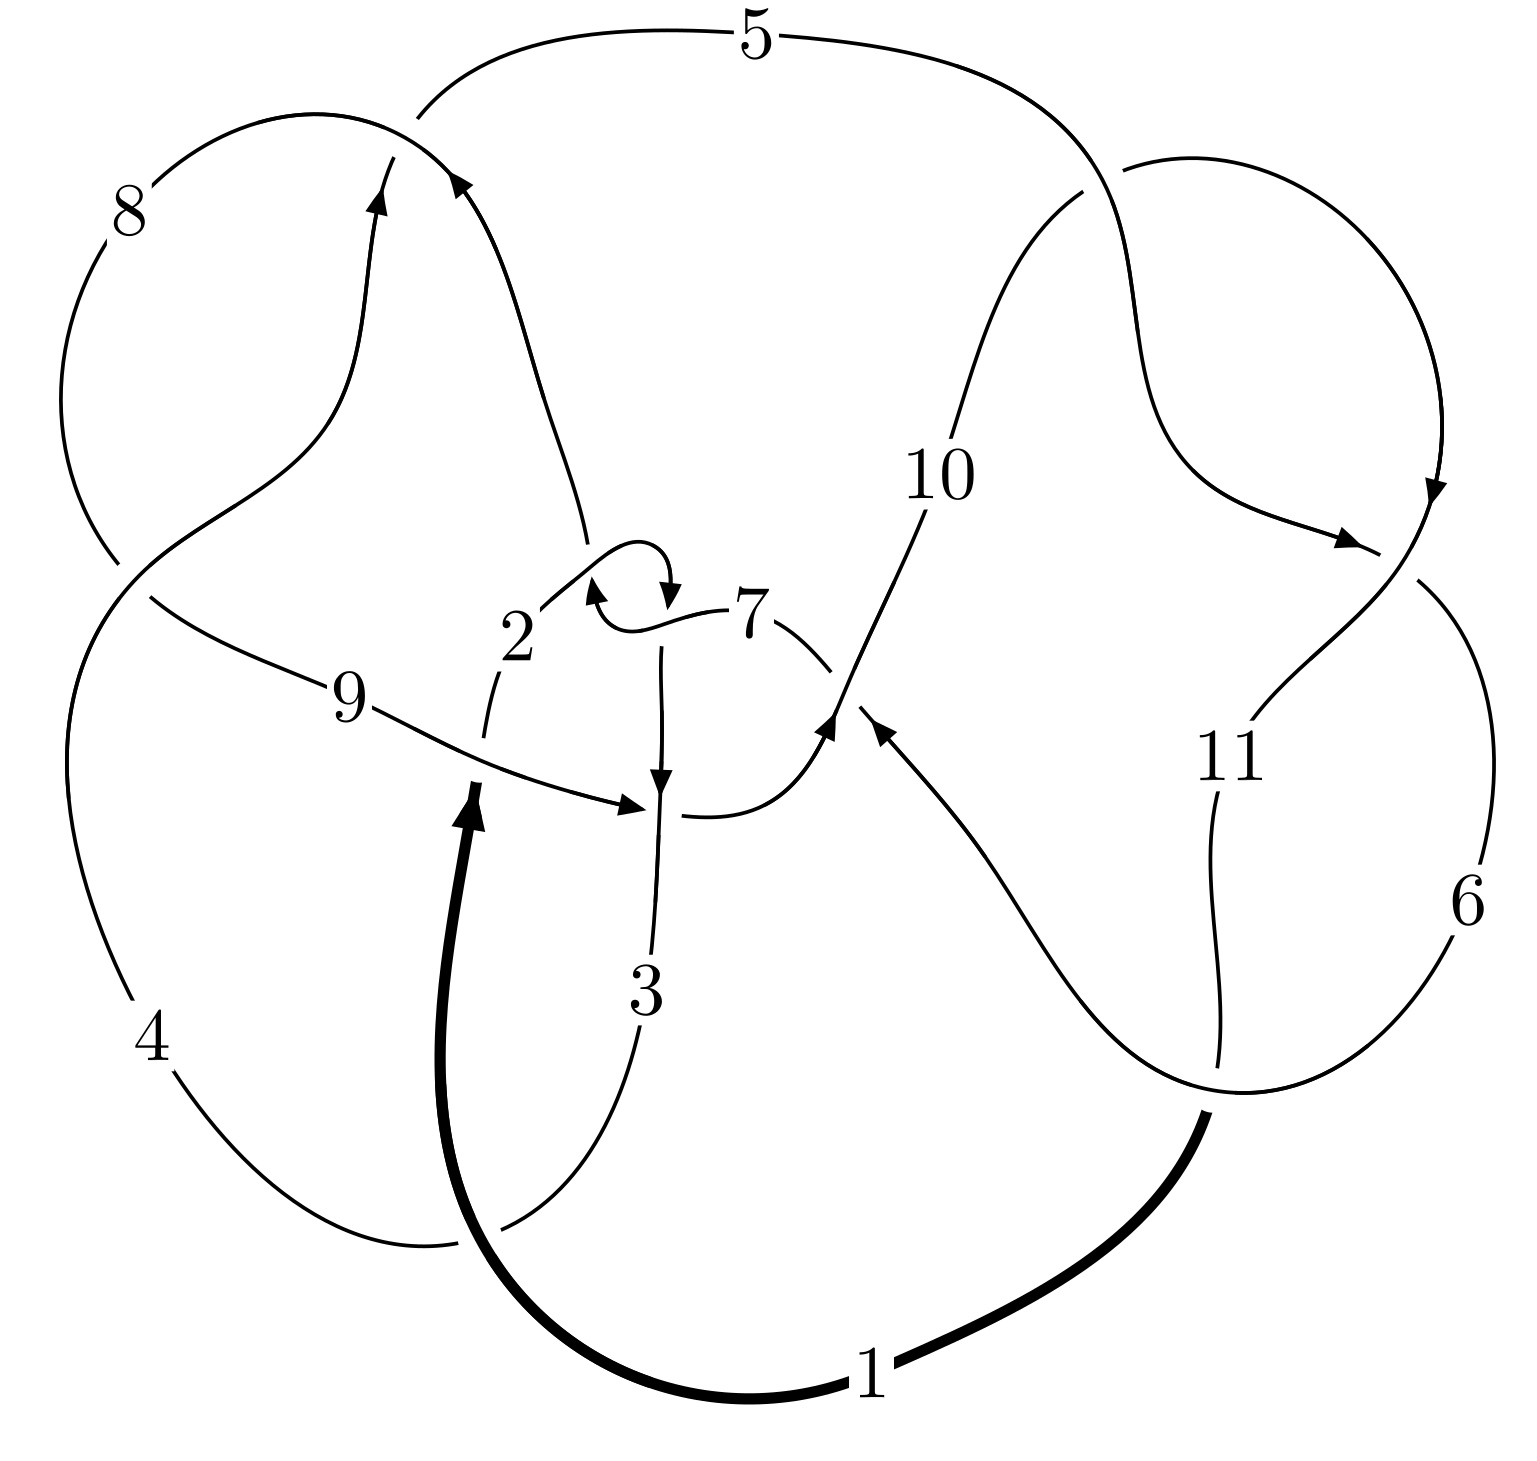
\includegraphics[width=112pt]{../../../GIT/diagram.site/Diagrams/png/593_11a_344.png}\\
\ \ \ A knot diagram\footnotemark}&
\allowdisplaybreaks
\textbf{Linearized knot diagam} \\
\cline{2-2}
 &
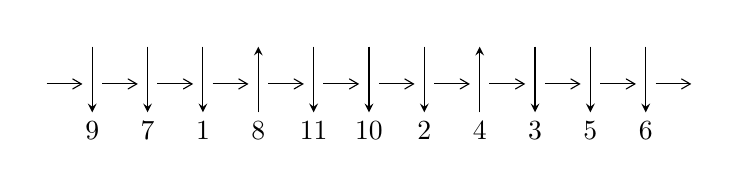
\begin{tikzpicture}[x=20pt, y=17pt]
	% nodes
	\node (C0) at (0, 0) {};
	\node (C1) at (1, 0) {};
	\node (C1U) at (1, +1) {};
	\node (C1D) at (1, -1) {9};

	\node (C2) at (2, 0) {};
	\node (C2U) at (2, +1) {};
	\node (C2D) at (2, -1) {7};

	\node (C3) at (3, 0) {};
	\node (C3U) at (3, +1) {};
	\node (C3D) at (3, -1) {1};

	\node (C4) at (4, 0) {};
	\node (C4U) at (4, +1) {};
	\node (C4D) at (4, -1) {8};

	\node (C5) at (5, 0) {};
	\node (C5U) at (5, +1) {};
	\node (C5D) at (5, -1) {11};

	\node (C6) at (6, 0) {};
	\node (C6U) at (6, +1) {};
	\node (C6D) at (6, -1) {10};

	\node (C7) at (7, 0) {};
	\node (C7U) at (7, +1) {};
	\node (C7D) at (7, -1) {2};

	\node (C8) at (8, 0) {};
	\node (C8U) at (8, +1) {};
	\node (C8D) at (8, -1) {4};

	\node (C9) at (9, 0) {};
	\node (C9U) at (9, +1) {};
	\node (C9D) at (9, -1) {3};

	\node (C10) at (10, 0) {};
	\node (C10U) at (10, +1) {};
	\node (C10D) at (10, -1) {5};

	\node (C11) at (11, 0) {};
	\node (C11U) at (11, +1) {};
	\node (C11D) at (11, -1) {6};
	\node (C12) at (12, 0) {};

	% arrows
	\draw[->,>={angle 60}]
	(C0) edge (C1) (C1) edge (C2) (C2) edge (C3) (C3) edge (C4) (C4) edge (C5) (C5) edge (C6) (C6) edge (C7) (C7) edge (C8) (C8) edge (C9) (C9) edge (C10) (C10) edge (C11) (C11) edge (C12) ;	\draw[->,>=stealth]
	(C1U) edge (C1D) (C2U) edge (C2D) (C3U) edge (C3D) (C4D) edge (C4U) (C5U) edge (C5D) (C6U) edge (C6D) (C7U) edge (C7D) (C8D) edge (C8U) (C9U) edge (C9D) (C10U) edge (C10D) (C11U) edge (C11D) ;
	\end{tikzpicture} \\
\hhline{~~} \\& 
\textbf{Solving Sequence} \\ \cline{2-2} 
 &
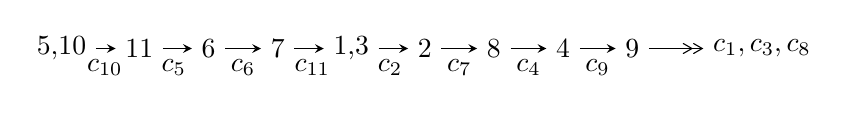
\begin{tikzpicture}[x=25pt, y=7pt]
	% node
	\node (A0) at (-1/8, 0) {5,10};
	\node (A1) at (1, 0) {11};
	\node (A2) at (2, 0) {6};
	\node (A3) at (3, 0) {7};
	\node (A4) at (65/16, 0) {1,3};
	\node (A5) at (41/8, 0) {2};
	\node (A6) at (49/8, 0) {8};
	\node (A7) at (57/8, 0) {4};
	\node (A8) at (65/8, 0) {9};
	\node (C1) at (1/2, -1) {$c_{10}$};
	\node (C2) at (3/2, -1) {$c_{5}$};
	\node (C3) at (5/2, -1) {$c_{6}$};
	\node (C4) at (7/2, -1) {$c_{11}$};
	\node (C5) at (37/8, -1) {$c_{2}$};
	\node (C6) at (45/8, -1) {$c_{7}$};
	\node (C7) at (53/8, -1) {$c_{4}$};
	\node (C8) at (61/8, -1) {$c_{9}$};
	\node (A9) at (10, 0) {$c_{1},c_{3},c_{8}$};

	% edge
	\draw[->,>=stealth]	
	(A0) edge (A1) (A1) edge (A2) (A2) edge (A3) (A3) edge (A4) (A4) edge (A5) (A5) edge (A6) (A6) edge (A7) (A7) edge (A8) ;
	\draw[->>,>={angle 60}]	
	(A8) edge (A9);
\end{tikzpicture} \\ 

\end{tabular} \\

\footnotetext{
The image of knot diagram is generated by the software ``\textbf{Draw programme}" developed by Andrew Bartholomew(\url{http://www.layer8.co.uk/maths/draw/index.htm\#Running-draw}), where we modified some parts for our purpose(\url{https://github.com/CATsTAILs/LinksPainter}).
}\phantom \\ \newline 
\centering \textbf{Ideals for irreducible components\footnotemark of $X_{\text{par}}$} 
 
\begin{align*}
I^u_{1}&=\langle 
-3.87710\times10^{61} u^{75}+3.95359\times10^{60} u^{74}+\cdots+4.66648\times10^{61} b+9.74216\times10^{61},\\
\phantom{I^u_{1}}&\phantom{= \langle  }-1.83090\times10^{62} u^{75}+2.54599\times10^{61} u^{74}+\cdots+3.26653\times10^{62} a+2.76516\times10^{62},\;u^{76}+u^{75}+\cdots-12 u-7\rangle \\
I^u_{2}&=\langle 
- u^7+3 u^5-2 u^3+u^2+b- u-1,\;u^{11}- u^{10}-5 u^9+4 u^8+9 u^7-5 u^6-5 u^5+u^4-2 u^3- u^2+a+u+4,\\
\phantom{I^u_{2}}&\phantom{= \langle  }u^{12}-6 u^{10}+13 u^8- u^7-10 u^6+4 u^5-2 u^4-5 u^3+4 u^2+2 u+1\rangle \\
\\
\end{align*}
\raggedright * 2 irreducible components of $\dim_{\mathbb{C}}=0$, with total 88 representations.\\
\footnotetext{All coefficients of polynomials are rational numbers. But the coefficients are sometimes approximated in decimal forms when there is not enough margin.}
\newpage
\renewcommand{\arraystretch}{1}
\centering \section*{I. $I^u_{1}= \langle -3.88\times10^{61} u^{75}+3.95\times10^{60} u^{74}+\cdots+4.67\times10^{61} b+9.74\times10^{61},\;-1.83\times10^{62} u^{75}+2.55\times10^{61} u^{74}+\cdots+3.27\times10^{62} a+2.77\times10^{62},\;u^{76}+u^{75}+\cdots-12 u-7 \rangle$}
\flushleft \textbf{(i) Arc colorings}\\
\begin{tabular}{m{7pt} m{180pt} m{7pt} m{180pt} }
\flushright $a_{5}=$&$\begin{pmatrix}0\\u\end{pmatrix}$ \\
\flushright $a_{10}=$&$\begin{pmatrix}1\\0\end{pmatrix}$ \\
\flushright $a_{11}=$&$\begin{pmatrix}1\\u^2\end{pmatrix}$ \\
\flushright $a_{6}=$&$\begin{pmatrix}- u\\- u^3+u\end{pmatrix}$ \\
\flushright $a_{7}=$&$\begin{pmatrix}u^3-2 u\\- u^3+u\end{pmatrix}$ \\
\flushright $a_{1}=$&$\begin{pmatrix}- u^2+1\\- u^4+2 u^2\end{pmatrix}$ \\
\flushright $a_{3}=$&$\begin{pmatrix}0.560502 u^{75}-0.0779417 u^{74}+\cdots-9.59790 u-0.846512\\0.830840 u^{75}-0.0847233 u^{74}+\cdots-1.54729 u-2.08769\end{pmatrix}$ \\
\flushright $a_{2}=$&$\begin{pmatrix}-0.329680 u^{75}-0.0658791 u^{74}+\cdots-7.74953 u+0.366663\\1.74221 u^{75}-0.275080 u^{74}+\cdots-3.59422 u-3.39247\end{pmatrix}$ \\
\flushright $a_{8}=$&$\begin{pmatrix}0.535153 u^{75}-0.116974 u^{74}+\cdots-4.19208 u-8.38576\\-0.960929 u^{75}+0.121521 u^{74}+\cdots+6.18648 u+6.54630\end{pmatrix}$ \\
\flushright $a_{4}=$&$\begin{pmatrix}-0.315830 u^{75}+0.0000729843 u^{74}+\cdots-8.58111 u+1.08231\\1.95879 u^{75}-0.464009 u^{74}+\cdots-5.04491 u-5.66772\end{pmatrix}$ \\
\flushright $a_{9}=$&$\begin{pmatrix}0.128996 u^{75}+0.0215062 u^{74}+\cdots-10.2764 u+4.42926\\1.77769 u^{75}-0.255216 u^{74}+\cdots-8.27842 u-11.8010\end{pmatrix}$\\ \flushright $a_{9}=$&$\begin{pmatrix}0.128996 u^{75}+0.0215062 u^{74}+\cdots-10.2764 u+4.42926\\1.77769 u^{75}-0.255216 u^{74}+\cdots-8.27842 u-11.8010\end{pmatrix}$\\&\end{tabular}
\flushleft \textbf{(ii) Obstruction class $= -1$}\\~\\
\flushleft \textbf{(iii) Cusp Shapes $= -0.332173 u^{75}+1.45404 u^{74}+\cdots-12.2591 u-8.45946$}\\~\\
\newpage\renewcommand{\arraystretch}{1}
\flushleft \textbf{(iv) u-Polynomials at the component}\newline \\
\begin{tabular}{m{50pt}|m{274pt}}
Crossings & \hspace{64pt}u-Polynomials at each crossing \\
\hline $$\begin{aligned}c_{1}\end{aligned}$$&$\begin{aligned}
&u^{76}+5 u^{75}+\cdots+u-2
\end{aligned}$\\
\hline $$\begin{aligned}c_{2},c_{7}\end{aligned}$$&$\begin{aligned}
&u^{76}- u^{75}+\cdots-23 u-101
\end{aligned}$\\
\hline $$\begin{aligned}c_{3}\end{aligned}$$&$\begin{aligned}
&u^{76}-11 u^{75}+\cdots+9 u+11
\end{aligned}$\\
\hline $$\begin{aligned}c_{4},c_{8}\end{aligned}$$&$\begin{aligned}
&u^{76}-2 u^{75}+\cdots+198 u-29
\end{aligned}$\\
\hline $$\begin{aligned}c_{5},c_{10},c_{11}\end{aligned}$$&$\begin{aligned}
&u^{76}- u^{75}+\cdots+12 u-7
\end{aligned}$\\
\hline $$\begin{aligned}c_{6}\end{aligned}$$&$\begin{aligned}
&u^{76}+3 u^{75}+\cdots-3283 u+4312
\end{aligned}$\\
\hline $$\begin{aligned}c_{9}\end{aligned}$$&$\begin{aligned}
&u^{76}+7 u^{74}+\cdots-7948 u-1013
\end{aligned}$\\
\hline
\end{tabular}\\~\\
\newpage\renewcommand{\arraystretch}{1}
\flushleft \textbf{(v) Riley Polynomials at the component}\newline \\
\begin{tabular}{m{50pt}|m{274pt}}
Crossings & \hspace{64pt}Riley Polynomials at each crossing \\
\hline $$\begin{aligned}c_{1}\end{aligned}$$&$\begin{aligned}
&y^{76}-3 y^{75}+\cdots+63 y+4
\end{aligned}$\\
\hline $$\begin{aligned}c_{2},c_{7}\end{aligned}$$&$\begin{aligned}
&y^{76}+53 y^{75}+\cdots+200865 y+10201
\end{aligned}$\\
\hline $$\begin{aligned}c_{3}\end{aligned}$$&$\begin{aligned}
&y^{76}-11 y^{75}+\cdots-2567 y+121
\end{aligned}$\\
\hline $$\begin{aligned}c_{4},c_{8}\end{aligned}$$&$\begin{aligned}
&y^{76}+46 y^{75}+\cdots-29344 y+841
\end{aligned}$\\
\hline $$\begin{aligned}c_{5},c_{10},c_{11}\end{aligned}$$&$\begin{aligned}
&y^{76}-67 y^{75}+\cdots+500 y+49
\end{aligned}$\\
\hline $$\begin{aligned}c_{6}\end{aligned}$$&$\begin{aligned}
&y^{76}+25 y^{75}+\cdots-18824281 y+18593344
\end{aligned}$\\
\hline $$\begin{aligned}c_{9}\end{aligned}$$&$\begin{aligned}
&y^{76}+14 y^{75}+\cdots+25053492 y+1026169
\end{aligned}$\\
\hline
\end{tabular}\\~\\
\newpage\flushleft \textbf{(vi) Complex Volumes and Cusp Shapes}
$$\begin{array}{c|c|c}  
\text{Solutions to }I^u_{1}& \I (\text{vol} + \sqrt{-1}CS) & \text{Cusp shape}\\
 \hline 
\begin{aligned}
u &= -0.968679 + 0.306013 I \\
a &= \phantom{-}0.936744 + 0.290091 I \\
b &= -0.54901 - 1.35285 I\end{aligned}
 & \phantom{-}3.49997 - 1.86931 I & \phantom{-0.000000 } 0 \\ \hline\begin{aligned}
u &= -0.968679 - 0.306013 I \\
a &= \phantom{-}0.936744 - 0.290091 I \\
b &= -0.54901 + 1.35285 I\end{aligned}
 & \phantom{-}3.49997 + 1.86931 I & \phantom{-0.000000 } 0 \\ \hline\begin{aligned}
u &= -0.402726 + 0.858164 I \\
a &= -0.228589 - 0.621929 I \\
b &= -0.323000 + 0.715407 I\end{aligned}
 & \phantom{-}3.74004 + 2.56276 I & \phantom{-0.000000 } 0. - 11.02950 I \\ \hline\begin{aligned}
u &= -0.402726 - 0.858164 I \\
a &= -0.228589 + 0.621929 I \\
b &= -0.323000 - 0.715407 I\end{aligned}
 & \phantom{-}3.74004 - 2.56276 I & \phantom{-0.000000 -}0. + 11.02950 I \\ \hline\begin{aligned}
u &= \phantom{-}0.150149 + 0.934780 I \\
a &= \phantom{-}0.047146 + 0.930784 I \\
b &= -0.424630 - 0.704027 I\end{aligned}
 & \phantom{-}3.32458 - 0.03587 I & -1.51662 + 0. I\phantom{ +0.000000I} \\ \hline\begin{aligned}
u &= \phantom{-}0.150149 - 0.934780 I \\
a &= \phantom{-}0.047146 - 0.930784 I \\
b &= -0.424630 + 0.704027 I\end{aligned}
 & \phantom{-}3.32458 + 0.03587 I & -1.51662 + 0. I\phantom{ +0.000000I} \\ \hline\begin{aligned}
u &= \phantom{-}0.931604 + 0.510293 I \\
a &= \phantom{-}0.912239 - 0.333719 I \\
b &= -0.686062 + 1.169450 I\end{aligned}
 & \phantom{-}0.53464 + 7.36666 I & \phantom{-0.000000 } 0 \\ \hline\begin{aligned}
u &= \phantom{-}0.931604 - 0.510293 I \\
a &= \phantom{-}0.912239 + 0.333719 I \\
b &= -0.686062 - 1.169450 I\end{aligned}
 & \phantom{-}0.53464 - 7.36666 I & \phantom{-0.000000 } 0 \\ \hline\begin{aligned}
u &= \phantom{-}0.248826 + 0.843265 I \\
a &= -0.23673 - 2.05712 I \\
b &= \phantom{-}0.89742 + 1.31819 I\end{aligned}
 & \phantom{-}2.65342 - 12.13500 I & -5.18296 + 8.02614 I \\ \hline\begin{aligned}
u &= \phantom{-}0.248826 - 0.843265 I \\
a &= -0.23673 + 2.05712 I \\
b &= \phantom{-}0.89742 - 1.31819 I\end{aligned}
 & \phantom{-}2.65342 + 12.13500 I & -5.18296 - 8.02614 I\\
 \hline 
 \end{array}$$\newpage$$\begin{array}{c|c|c}  
\text{Solutions to }I^u_{1}& \I (\text{vol} + \sqrt{-1}CS) & \text{Cusp shape}\\
 \hline 
\begin{aligned}
u &= \phantom{-}1.009890 + 0.581338 I \\
a &= -0.128172 + 0.337314 I \\
b &= -0.026272 - 0.785988 I\end{aligned}
 & \phantom{-}0.66505 - 5.23954 I & \phantom{-0.000000 } 0 \\ \hline\begin{aligned}
u &= \phantom{-}1.009890 - 0.581338 I \\
a &= -0.128172 - 0.337314 I \\
b &= -0.026272 + 0.785988 I\end{aligned}
 & \phantom{-}0.66505 + 5.23954 I & \phantom{-0.000000 } 0 \\ \hline\begin{aligned}
u &= -1.184460 + 0.087532 I \\
a &= -1.25675 - 1.30618 I \\
b &= \phantom{-}0.195439 + 0.281765 I\end{aligned}
 & -3.89513 - 3.10544 I & \phantom{-0.000000 } 0 \\ \hline\begin{aligned}
u &= -1.184460 - 0.087532 I \\
a &= -1.25675 + 1.30618 I \\
b &= \phantom{-}0.195439 - 0.281765 I\end{aligned}
 & -3.89513 + 3.10544 I & \phantom{-0.000000 } 0 \\ \hline\begin{aligned}
u &= -0.201569 + 0.767240 I \\
a &= -0.23031 + 2.38711 I \\
b &= \phantom{-}0.90138 - 1.50036 I\end{aligned}
 & \phantom{-}5.85346 + 5.89693 I & -1.84592 - 6.16015 I \\ \hline\begin{aligned}
u &= -0.201569 - 0.767240 I \\
a &= -0.23031 - 2.38711 I \\
b &= \phantom{-}0.90138 + 1.50036 I\end{aligned}
 & \phantom{-}5.85346 - 5.89693 I & -1.84592 + 6.16015 I \\ \hline\begin{aligned}
u &= \phantom{-}0.062116 + 0.761993 I \\
a &= -0.46367 + 1.82956 I \\
b &= -0.435791 - 0.829410 I\end{aligned}
 & \phantom{-}3.69493 - 3.40892 I & -2.10008 + 7.62336 I \\ \hline\begin{aligned}
u &= \phantom{-}0.062116 - 0.761993 I \\
a &= -0.46367 - 1.82956 I \\
b &= -0.435791 + 0.829410 I\end{aligned}
 & \phantom{-}3.69493 + 3.40892 I & -2.10008 - 7.62336 I \\ \hline\begin{aligned}
u &= \phantom{-}1.203070 + 0.312929 I \\
a &= -0.066873 + 0.897972 I \\
b &= \phantom{-}0.327385 - 0.987472 I\end{aligned}
 & \phantom{-}0.209490 - 0.491453 I & \phantom{-0.000000 } 0 \\ \hline\begin{aligned}
u &= \phantom{-}1.203070 - 0.312929 I \\
a &= -0.066873 - 0.897972 I \\
b &= \phantom{-}0.327385 + 0.987472 I\end{aligned}
 & \phantom{-}0.209490 + 0.491453 I & \phantom{-0.000000 } 0\\
 \hline 
 \end{array}$$\newpage$$\begin{array}{c|c|c}  
\text{Solutions to }I^u_{1}& \I (\text{vol} + \sqrt{-1}CS) & \text{Cusp shape}\\
 \hline 
\begin{aligned}
u &= \phantom{-}1.234810 + 0.206791 I \\
a &= -0.721753 + 0.756146 I \\
b &= \phantom{-}0.135004 - 0.637912 I\end{aligned}
 & -1.62348 - 1.28005 I & \phantom{-0.000000 } 0 \\ \hline\begin{aligned}
u &= \phantom{-}1.234810 - 0.206791 I \\
a &= -0.721753 - 0.756146 I \\
b &= \phantom{-}0.135004 + 0.637912 I\end{aligned}
 & -1.62348 + 1.28005 I & \phantom{-0.000000 } 0 \\ \hline\begin{aligned}
u &= -0.211230 + 0.692166 I \\
a &= \phantom{-}0.32479 - 2.42437 I \\
b &= -0.579010 + 0.798991 I\end{aligned}
 & -1.61113 + 5.99074 I & -7.07123 - 7.64863 I \\ \hline\begin{aligned}
u &= -0.211230 - 0.692166 I \\
a &= \phantom{-}0.32479 + 2.42437 I \\
b &= -0.579010 - 0.798991 I\end{aligned}
 & -1.61113 - 5.99074 I & -7.07123 + 7.64863 I \\ \hline\begin{aligned}
u &= -1.264020 + 0.200993 I \\
a &= -0.743336 - 1.099380 I \\
b &= -1.81254 + 0.02250 I\end{aligned}
 & -3.68056 - 0.68832 I & \phantom{-0.000000 } 0 \\ \hline\begin{aligned}
u &= -1.264020 - 0.200993 I \\
a &= -0.743336 + 1.099380 I \\
b &= -1.81254 - 0.02250 I\end{aligned}
 & -3.68056 + 0.68832 I & \phantom{-0.000000 } 0 \\ \hline\begin{aligned}
u &= -0.637024 + 0.316684 I \\
a &= -0.0814032 + 0.0833784 I \\
b &= -0.235620 + 0.937335 I\end{aligned}
 & \phantom{-}3.01317 + 1.73011 I & -2.31903 - 3.39119 I \\ \hline\begin{aligned}
u &= -0.637024 - 0.316684 I \\
a &= -0.0814032 - 0.0833784 I \\
b &= -0.235620 - 0.937335 I\end{aligned}
 & \phantom{-}3.01317 - 1.73011 I & -2.31903 + 3.39119 I \\ \hline\begin{aligned}
u &= -1.284140 + 0.219366 I \\
a &= \phantom{-}0.183447 - 1.023270 I \\
b &= \phantom{-}0.352547 + 1.162330 I\end{aligned}
 & \phantom{-}0.12887 + 2.52959 I & \phantom{-0.000000 } 0 \\ \hline\begin{aligned}
u &= -1.284140 - 0.219366 I \\
a &= \phantom{-}0.183447 + 1.023270 I \\
b &= \phantom{-}0.352547 - 1.162330 I\end{aligned}
 & \phantom{-}0.12887 - 2.52959 I & \phantom{-0.000000 } 0\\
 \hline 
 \end{array}$$\newpage$$\begin{array}{c|c|c}  
\text{Solutions to }I^u_{1}& \I (\text{vol} + \sqrt{-1}CS) & \text{Cusp shape}\\
 \hline 
\begin{aligned}
u &= \phantom{-}0.075482 + 0.672046 I \\
a &= \phantom{-}0.64227 + 1.93805 I \\
b &= -0.534886 - 0.748714 I\end{aligned}
 & \phantom{-}1.83137 - 1.88031 I & -3.15463 + 4.07325 I \\ \hline\begin{aligned}
u &= \phantom{-}0.075482 - 0.672046 I \\
a &= \phantom{-}0.64227 - 1.93805 I \\
b &= -0.534886 + 0.748714 I\end{aligned}
 & \phantom{-}1.83137 + 1.88031 I & -3.15463 - 4.07325 I \\ \hline\begin{aligned}
u &= \phantom{-}0.369901 + 0.560002 I \\
a &= \phantom{-}1.17517 - 0.88223 I \\
b &= -0.380653 + 0.890018 I\end{aligned}
 & -1.20192 - 1.77591 I & -8.18323 + 1.57822 I \\ \hline\begin{aligned}
u &= \phantom{-}0.369901 - 0.560002 I \\
a &= \phantom{-}1.17517 + 0.88223 I \\
b &= -0.380653 - 0.890018 I\end{aligned}
 & -1.20192 + 1.77591 I & -8.18323 - 1.57822 I \\ \hline\begin{aligned}
u &= \phantom{-}1.310420 + 0.247828 I \\
a &= \phantom{-}1.47529 - 0.24769 I \\
b &= \phantom{-}0.571098 + 0.537826 I\end{aligned}
 & -0.27749 - 3.56587 I & \phantom{-0.000000 } 0 \\ \hline\begin{aligned}
u &= \phantom{-}1.310420 - 0.247828 I \\
a &= \phantom{-}1.47529 + 0.24769 I \\
b &= \phantom{-}0.571098 - 0.537826 I\end{aligned}
 & -0.27749 + 3.56587 I & \phantom{-0.000000 } 0 \\ \hline\begin{aligned}
u &= -1.33405\phantom{ +0.000000I} \\
a &= -0.863799\phantom{ +0.000000I} \\
b &= -1.01726\phantom{ +0.000000I}\end{aligned}
 & -5.87122\phantom{ +0.000000I} & \phantom{-0.000000 } 0 \\ \hline\begin{aligned}
u &= \phantom{-}1.325920 + 0.160373 I \\
a &= \phantom{-}0.78766 - 1.54148 I \\
b &= \phantom{-}0.93014 + 1.41946 I\end{aligned}
 & -5.55889 + 0.47303 I & \phantom{-0.000000 } 0 \\ \hline\begin{aligned}
u &= \phantom{-}1.325920 - 0.160373 I \\
a &= \phantom{-}0.78766 + 1.54148 I \\
b &= \phantom{-}0.93014 - 1.41946 I\end{aligned}
 & -5.55889 - 0.47303 I & \phantom{-0.000000 } 0 \\ \hline\begin{aligned}
u &= -1.308300 + 0.270202 I \\
a &= \phantom{-}0.64800 + 1.41204 I \\
b &= \phantom{-}0.832561 - 0.888141 I\end{aligned}
 & -2.49885 + 5.30835 I & \phantom{-0.000000 } 0\\
 \hline 
 \end{array}$$\newpage$$\begin{array}{c|c|c}  
\text{Solutions to }I^u_{1}& \I (\text{vol} + \sqrt{-1}CS) & \text{Cusp shape}\\
 \hline 
\begin{aligned}
u &= -1.308300 - 0.270202 I \\
a &= \phantom{-}0.64800 - 1.41204 I \\
b &= \phantom{-}0.832561 + 0.888141 I\end{aligned}
 & -2.49885 - 5.30835 I & \phantom{-0.000000 } 0 \\ \hline\begin{aligned}
u &= -1.305040 + 0.319754 I \\
a &= \phantom{-}1.38303 + 0.97569 I \\
b &= \phantom{-}0.543065 - 0.675937 I\end{aligned}
 & -0.57872 + 7.31208 I & \phantom{-0.000000 } 0 \\ \hline\begin{aligned}
u &= -1.305040 - 0.319754 I \\
a &= \phantom{-}1.38303 - 0.97569 I \\
b &= \phantom{-}0.543065 + 0.675937 I\end{aligned}
 & -0.57872 - 7.31208 I & \phantom{-0.000000 } 0 \\ \hline\begin{aligned}
u &= \phantom{-}1.327950 + 0.244567 I \\
a &= \phantom{-}0.244688 + 0.775435 I \\
b &= -1.90753 + 0.89944 I\end{aligned}
 & -4.47754 - 6.67234 I & \phantom{-0.000000 } 0 \\ \hline\begin{aligned}
u &= \phantom{-}1.327950 - 0.244567 I \\
a &= \phantom{-}0.244688 - 0.775435 I \\
b &= -1.90753 - 0.89944 I\end{aligned}
 & -4.47754 + 6.67234 I & \phantom{-0.000000 } 0 \\ \hline\begin{aligned}
u &= -0.564347 + 0.281716 I \\
a &= -0.419798 - 0.783383 I \\
b &= \phantom{-}0.808778 + 0.477749 I\end{aligned}
 & -3.26194 - 2.66752 I & -12.49560 + 1.19911 I \\ \hline\begin{aligned}
u &= -0.564347 - 0.281716 I \\
a &= -0.419798 + 0.783383 I \\
b &= \phantom{-}0.808778 - 0.477749 I\end{aligned}
 & -3.26194 + 2.66752 I & -12.49560 - 1.19911 I \\ \hline\begin{aligned}
u &= \phantom{-}0.368179 + 0.508001 I \\
a &= \phantom{-}0.96836 - 1.48644 I \\
b &= \phantom{-}0.126296 + 1.052670 I\end{aligned}
 & -1.29394 - 1.64438 I & -9.75127 + 4.13442 I \\ \hline\begin{aligned}
u &= \phantom{-}0.368179 - 0.508001 I \\
a &= \phantom{-}0.96836 + 1.48644 I \\
b &= \phantom{-}0.126296 - 1.052670 I\end{aligned}
 & -1.29394 + 1.64438 I & -9.75127 - 4.13442 I \\ \hline\begin{aligned}
u &= -0.075467 + 0.609557 I \\
a &= -1.85586 - 0.84943 I \\
b &= \phantom{-}1.75807 + 0.52628 I\end{aligned}
 & -0.03422 + 3.55485 I & -4.57668 - 5.47640 I\\
 \hline 
 \end{array}$$\newpage$$\begin{array}{c|c|c}  
\text{Solutions to }I^u_{1}& \I (\text{vol} + \sqrt{-1}CS) & \text{Cusp shape}\\
 \hline 
\begin{aligned}
u &= -0.075467 - 0.609557 I \\
a &= -1.85586 + 0.84943 I \\
b &= \phantom{-}1.75807 - 0.52628 I\end{aligned}
 & -0.03422 - 3.55485 I & -4.57668 + 5.47640 I \\ \hline\begin{aligned}
u &= -0.044203 + 0.612297 I \\
a &= -1.23990 - 1.62222 I \\
b &= -0.389998 + 0.831508 I\end{aligned}
 & \phantom{-}4.00054 + 0.42281 I & -1.53362 + 1.17105 I \\ \hline\begin{aligned}
u &= -0.044203 - 0.612297 I \\
a &= -1.23990 + 1.62222 I \\
b &= -0.389998 - 0.831508 I\end{aligned}
 & \phantom{-}4.00054 - 0.42281 I & -1.53362 - 1.17105 I \\ \hline\begin{aligned}
u &= \phantom{-}1.389280 + 0.027409 I \\
a &= \phantom{-}0.100143 - 0.840012 I \\
b &= \phantom{-}0.943148 - 0.485048 I\end{aligned}
 & -3.13133 + 2.04238 I & \phantom{-0.000000 } 0 \\ \hline\begin{aligned}
u &= \phantom{-}1.389280 - 0.027409 I \\
a &= \phantom{-}0.100143 + 0.840012 I \\
b &= \phantom{-}0.943148 + 0.485048 I\end{aligned}
 & -3.13133 - 2.04238 I & \phantom{-0.000000 } 0 \\ \hline\begin{aligned}
u &= -1.334670 + 0.401679 I \\
a &= \phantom{-}0.525115 + 0.884565 I \\
b &= \phantom{-}0.751457 - 0.668315 I\end{aligned}
 & -1.28728 + 4.79520 I & \phantom{-0.000000 } 0 \\ \hline\begin{aligned}
u &= -1.334670 - 0.401679 I \\
a &= \phantom{-}0.525115 - 0.884565 I \\
b &= \phantom{-}0.751457 + 0.668315 I\end{aligned}
 & -1.28728 - 4.79520 I & \phantom{-0.000000 } 0 \\ \hline\begin{aligned}
u &= \phantom{-}1.379300 + 0.285950 I \\
a &= \phantom{-}0.77351 - 1.51750 I \\
b &= \phantom{-}0.669261 + 1.000640 I\end{aligned}
 & -6.65323 - 9.56425 I & \phantom{-0.000000 } 0 \\ \hline\begin{aligned}
u &= \phantom{-}1.379300 - 0.285950 I \\
a &= \phantom{-}0.77351 + 1.51750 I \\
b &= \phantom{-}0.669261 - 1.000640 I\end{aligned}
 & -6.65323 + 9.56425 I & \phantom{-0.000000 } 0 \\ \hline\begin{aligned}
u &= \phantom{-}1.38264 + 0.31570 I \\
a &= -1.22325 + 1.23732 I \\
b &= -1.13602 - 1.53413 I\end{aligned}
 & \phantom{-}0.83133 - 9.81598 I & \phantom{-0.000000 } 0\\
 \hline 
 \end{array}$$\newpage$$\begin{array}{c|c|c}  
\text{Solutions to }I^u_{1}& \I (\text{vol} + \sqrt{-1}CS) & \text{Cusp shape}\\
 \hline 
\begin{aligned}
u &= \phantom{-}1.38264 - 0.31570 I \\
a &= -1.22325 - 1.23732 I \\
b &= -1.13602 + 1.53413 I\end{aligned}
 & \phantom{-}0.83133 + 9.81598 I & \phantom{-0.000000 } 0 \\ \hline\begin{aligned}
u &= -1.40631 + 0.21816 I \\
a &= -1.026610 - 0.485658 I \\
b &= -0.272085 + 1.269180 I\end{aligned}
 & -6.84634 + 4.36487 I & \phantom{-0.000000 } 0 \\ \hline\begin{aligned}
u &= -1.40631 - 0.21816 I \\
a &= -1.026610 + 0.485658 I \\
b &= -0.272085 - 1.269180 I\end{aligned}
 & -6.84634 - 4.36487 I & \phantom{-0.000000 } 0 \\ \hline\begin{aligned}
u &= \phantom{-}1.42980 + 0.07326 I \\
a &= -0.490884 - 0.045086 I \\
b &= -1.101020 + 0.554963 I\end{aligned}
 & -9.55152 + 1.46003 I & \phantom{-0.000000 } 0 \\ \hline\begin{aligned}
u &= \phantom{-}1.42980 - 0.07326 I \\
a &= -0.490884 + 0.045086 I \\
b &= -1.101020 - 0.554963 I\end{aligned}
 & -9.55152 - 1.46003 I & \phantom{-0.000000 } 0 \\ \hline\begin{aligned}
u &= -1.43258 + 0.21432 I \\
a &= -0.770404 + 0.141503 I \\
b &= \phantom{-}0.531412 + 1.110610 I\end{aligned}
 & -6.96863 + 4.63471 I & \phantom{-0.000000 } 0 \\ \hline\begin{aligned}
u &= -1.43258 - 0.21432 I \\
a &= -0.770404 - 0.141503 I \\
b &= \phantom{-}0.531412 - 1.110610 I\end{aligned}
 & -6.96863 - 4.63471 I & \phantom{-0.000000 } 0 \\ \hline\begin{aligned}
u &= -1.41403 + 0.34833 I \\
a &= -1.03057 - 1.23596 I \\
b &= -1.07132 + 1.35240 I\end{aligned}
 & -2.6277 + 16.4336 I & \phantom{-0.000000 } 0 \\ \hline\begin{aligned}
u &= -1.41403 - 0.34833 I \\
a &= -1.03057 + 1.23596 I \\
b &= -1.07132 - 1.35240 I\end{aligned}
 & -2.6277 - 16.4336 I & \phantom{-0.000000 } 0 \\ \hline\begin{aligned}
u &= \phantom{-}1.45271 + 0.36773 I \\
a &= \phantom{-}0.481096 - 0.525580 I \\
b &= \phantom{-}0.743722 + 0.594956 I\end{aligned}
 & -2.09696 - 7.08063 I & \phantom{-0.000000 } 0\\
 \hline 
 \end{array}$$\newpage$$\begin{array}{c|c|c}  
\text{Solutions to }I^u_{1}& \I (\text{vol} + \sqrt{-1}CS) & \text{Cusp shape}\\
 \hline 
\begin{aligned}
u &= \phantom{-}1.45271 - 0.36773 I \\
a &= \phantom{-}0.481096 + 0.525580 I \\
b &= \phantom{-}0.743722 - 0.594956 I\end{aligned}
 & -2.09696 + 7.08063 I & \phantom{-0.000000 } 0 \\ \hline\begin{aligned}
u &= -1.53494 + 0.03855 I \\
a &= \phantom{-}0.132344 - 0.251214 I \\
b &= \phantom{-}0.750588 - 0.550715 I\end{aligned}
 & -8.13102 + 6.65132 I & \phantom{-0.000000 } 0 \\ \hline\begin{aligned}
u &= -1.53494 - 0.03855 I \\
a &= \phantom{-}0.132344 + 0.251214 I \\
b &= \phantom{-}0.750588 + 0.550715 I\end{aligned}
 & -8.13102 - 6.65132 I & \phantom{-0.000000 } 0 \\ \hline\begin{aligned}
u &= \phantom{-}0.375740\phantom{ +0.000000I} \\
a &= \phantom{-}0.100271\phantom{ +0.000000I} \\
b &= \phantom{-}0.540684\phantom{ +0.000000I}\end{aligned}
 & -0.725667\phantom{ +0.000000I} & -13.9610\phantom{ +0.000000I} \\ \hline\begin{aligned}
u &= -0.099162 + 0.335506 I \\
a &= \phantom{-}2.71273 - 3.59350 I \\
b &= -0.665037 + 0.775565 I\end{aligned}
 & -1.09766 - 2.44518 I & -6.25239 - 1.93768 I \\ \hline\begin{aligned}
u &= -0.099162 - 0.335506 I \\
a &= \phantom{-}2.71273 + 3.59350 I \\
b &= -0.665037 - 0.775565 I\end{aligned}
 & -1.09766 + 2.44518 I & -6.25239 + 1.93768 I\\
 \hline 
 \end{array}$$\newpage\newpage\renewcommand{\arraystretch}{1}
\centering \section*{II. $I^u_{2}= \langle - u^7+3 u^5-2 u^3+u^2+b- u-1,\;u^{11}- u^{10}+\cdots+a+4,\;u^{12}-6 u^{10}+\cdots+2 u+1 \rangle$}
\flushleft \textbf{(i) Arc colorings}\\
\begin{tabular}{m{7pt} m{180pt} m{7pt} m{180pt} }
\flushright $a_{5}=$&$\begin{pmatrix}0\\u\end{pmatrix}$ \\
\flushright $a_{10}=$&$\begin{pmatrix}1\\0\end{pmatrix}$ \\
\flushright $a_{11}=$&$\begin{pmatrix}1\\u^2\end{pmatrix}$ \\
\flushright $a_{6}=$&$\begin{pmatrix}- u\\- u^3+u\end{pmatrix}$ \\
\flushright $a_{7}=$&$\begin{pmatrix}u^3-2 u\\- u^3+u\end{pmatrix}$ \\
\flushright $a_{1}=$&$\begin{pmatrix}- u^2+1\\- u^4+2 u^2\end{pmatrix}$ \\
\flushright $a_{3}=$&$\begin{pmatrix}- u^{11}+u^{10}+5 u^9-4 u^8-9 u^7+5 u^6+5 u^5- u^4+2 u^3+u^2- u-4\\u^7-3 u^5+2 u^3- u^2+u+1\end{pmatrix}$ \\
\flushright $a_{2}=$&$\begin{pmatrix}- u^{11}+5 u^9+u^8-9 u^7-3 u^6+6 u^5+2 u^4- u^3+2 u^2+u-3\\u^7-3 u^5- u^4+2 u^3+u^2+u+1\end{pmatrix}$ \\
\flushright $a_{8}=$&$\begin{pmatrix}- u^{11}+u^{10}+6 u^9-5 u^8-13 u^7+10 u^6+9 u^5-9 u^4+5 u^3+3 u^2-7 u\\u^{11}+u^{10}-5 u^9-4 u^8+8 u^7+3 u^6-4 u^5+5 u^4-5 u^2-1\end{pmatrix}$ \\
\flushright $a_{4}=$&$\begin{pmatrix}- u^{11}+5 u^9+u^8-9 u^7-3 u^6+6 u^5+2 u^4- u^3+3 u^2+u-4\\u^{10}-4 u^8+u^7+5 u^6-4 u^5- u^4+4 u^3-2 u^2+u+1\end{pmatrix}$ \\
\flushright $a_{9}=$&$\begin{pmatrix}u^{10}-2 u^9-5 u^8+9 u^7+8 u^6-14 u^5+6 u^3-9 u^2+3 u+4\\u^9-4 u^7+5 u^5- u^4+2 u^2-2 u-1\end{pmatrix}$\\ \flushright $a_{9}=$&$\begin{pmatrix}u^{10}-2 u^9-5 u^8+9 u^7+8 u^6-14 u^5+6 u^3-9 u^2+3 u+4\\u^9-4 u^7+5 u^5- u^4+2 u^2-2 u-1\end{pmatrix}$\\&\end{tabular}
\flushleft \textbf{(ii) Obstruction class $= 1$}\\~\\
\flushleft \textbf{(iii) Cusp Shapes $= - u^{11}+12 u^9- u^8-36 u^7+6 u^6+37 u^5-16 u^4+2 u^3+16 u^2-15 u-12$}\\~\\
\newpage\renewcommand{\arraystretch}{1}
\flushleft \textbf{(iv) u-Polynomials at the component}\newline \\
\begin{tabular}{m{50pt}|m{274pt}}
Crossings & \hspace{64pt}u-Polynomials at each crossing \\
\hline $$\begin{aligned}c_{1}\end{aligned}$$&$\begin{aligned}
&u^{12}+2 u^9+2 u^8- u^7- u^5+u^4+u^3- u^2- u+1
\end{aligned}$\\
\hline $$\begin{aligned}c_{2}\end{aligned}$$&$\begin{aligned}
&u^{12}+6 u^{10}+u^9+14 u^8+4 u^7+17 u^6+6 u^5+12 u^4+3 u^3+5 u^2+u+1
\end{aligned}$\\
\hline $$\begin{aligned}c_{3}\end{aligned}$$&$\begin{aligned}
&u^{12}-2 u^{10}- u^9+2 u^8+2 u^7+3 u^6+4 u^5+2 u^4+u^3+3 u^2+3 u+1
\end{aligned}$\\
\hline $$\begin{aligned}c_{4}\end{aligned}$$&$\begin{aligned}
&u^{12}- u^{11}+5 u^{10}-3 u^9+12 u^8-6 u^7+17 u^6-4 u^5+14 u^4- u^3+6 u^2+1
\end{aligned}$\\
\hline $$\begin{aligned}c_{5}\end{aligned}$$&$\begin{aligned}
&u^{12}-6 u^{10}+13 u^8+u^7-10 u^6-4 u^5-2 u^4+5 u^3+4 u^2-2 u+1
\end{aligned}$\\
\hline $$\begin{aligned}c_{6}\end{aligned}$$&$\begin{aligned}
&u^{12}+2 u^{10}-3 u^9+4 u^8+4 u^7+12 u^6+7 u^5+3 u^4+4 u^3+4 u^2-2 u+1
\end{aligned}$\\
\hline $$\begin{aligned}c_{7}\end{aligned}$$&$\begin{aligned}
&u^{12}+6 u^{10}- u^9+14 u^8-4 u^7+17 u^6-6 u^5+12 u^4-3 u^3+5 u^2- u+1
\end{aligned}$\\
\hline $$\begin{aligned}c_{8}\end{aligned}$$&$\begin{aligned}
&u^{12}+u^{11}+5 u^{10}+3 u^9+12 u^8+6 u^7+17 u^6+4 u^5+14 u^4+u^3+6 u^2+1
\end{aligned}$\\
\hline $$\begin{aligned}c_{9}\end{aligned}$$&$\begin{aligned}
&u^{12}+u^{11}- u^{10}- u^9+u^8+u^7+u^5+2 u^4-2 u^3+1
\end{aligned}$\\
\hline $$\begin{aligned}c_{10},c_{11}\end{aligned}$$&$\begin{aligned}
&u^{12}-6 u^{10}+13 u^8- u^7-10 u^6+4 u^5-2 u^4-5 u^3+4 u^2+2 u+1
\end{aligned}$\\
\hline
\end{tabular}\\~\\
\newpage\renewcommand{\arraystretch}{1}
\flushleft \textbf{(v) Riley Polynomials at the component}\newline \\
\begin{tabular}{m{50pt}|m{274pt}}
Crossings & \hspace{64pt}Riley Polynomials at each crossing \\
\hline $$\begin{aligned}c_{1}\end{aligned}$$&$\begin{aligned}
&y^{12}+4 y^{10}-4 y^9+10 y^8+y^7+y^5+5 y^4-5 y^3+5 y^2-3 y+1
\end{aligned}$\\
\hline $$\begin{aligned}c_{2},c_{7}\end{aligned}$$&$\begin{aligned}
&y^{12}+12 y^{11}+\cdots+9 y+1
\end{aligned}$\\
\hline $$\begin{aligned}c_{3}\end{aligned}$$&$\begin{aligned}
&y^{12}-4 y^{11}+8 y^{10}-3 y^9+14 y^7-7 y^6+6 y^5+6 y^4-7 y^3+7 y^2-3 y+1
\end{aligned}$\\
\hline $$\begin{aligned}c_{4},c_{8}\end{aligned}$$&$\begin{aligned}
&y^{12}+9 y^{11}+\cdots+12 y+1
\end{aligned}$\\
\hline $$\begin{aligned}c_{5},c_{10},c_{11}\end{aligned}$$&$\begin{aligned}
&y^{12}-12 y^{11}+\cdots+4 y+1
\end{aligned}$\\
\hline $$\begin{aligned}c_{6}\end{aligned}$$&$\begin{aligned}
&y^{12}+4 y^{11}+\cdots+4 y+1
\end{aligned}$\\
\hline $$\begin{aligned}c_{9}\end{aligned}$$&$\begin{aligned}
&y^{12}-3 y^{11}+5 y^{10}-5 y^9+5 y^8+y^7+y^5+10 y^4-4 y^3+4 y^2+1
\end{aligned}$\\
\hline
\end{tabular}\\~\\
\newpage\flushleft \textbf{(vi) Complex Volumes and Cusp Shapes}
$$\begin{array}{c|c|c}  
\text{Solutions to }I^u_{2}& \I (\text{vol} + \sqrt{-1}CS) & \text{Cusp shape}\\
 \hline 
\begin{aligned}
u &= \phantom{-}0.215104 + 0.798845 I \\
a &= -0.413477 + 0.669068 I \\
b &= -0.377143 - 0.565754 I\end{aligned}
 & \phantom{-}3.50536 - 1.91915 I & -4.46198 + 0.73730 I \\ \hline\begin{aligned}
u &= \phantom{-}0.215104 - 0.798845 I \\
a &= -0.413477 - 0.669068 I \\
b &= -0.377143 + 0.565754 I\end{aligned}
 & \phantom{-}3.50536 + 1.91915 I & -4.46198 - 0.73730 I \\ \hline\begin{aligned}
u &= \phantom{-}1.181970 + 0.217891 I \\
a &= \phantom{-}0.539675 + 0.842839 I \\
b &= \phantom{-}0.241684 - 0.971815 I\end{aligned}
 & \phantom{-}0.83736 - 1.52744 I & -4.49507 + 0.61060 I \\ \hline\begin{aligned}
u &= \phantom{-}1.181970 - 0.217891 I \\
a &= \phantom{-}0.539675 - 0.842839 I \\
b &= \phantom{-}0.241684 + 0.971815 I\end{aligned}
 & \phantom{-}0.83736 + 1.52744 I & -4.49507 - 0.61060 I \\ \hline\begin{aligned}
u &= -1.286840 + 0.093791 I \\
a &= -0.86850 - 1.39935 I \\
b &= -1.299930 + 0.350855 I\end{aligned}
 & -4.83854 - 1.75409 I & -13.7193 + 4.0775 I \\ \hline\begin{aligned}
u &= -1.286840 - 0.093791 I \\
a &= -0.86850 + 1.39935 I \\
b &= -1.299930 - 0.350855 I\end{aligned}
 & -4.83854 + 1.75409 I & -13.7193 - 4.0775 I \\ \hline\begin{aligned}
u &= -1.334400 + 0.365970 I \\
a &= \phantom{-}0.637376 + 0.770937 I \\
b &= \phantom{-}0.740658 - 0.383732 I\end{aligned}
 & -1.29267 + 6.23322 I & -8.20976 - 5.43660 I \\ \hline\begin{aligned}
u &= -1.334400 - 0.365970 I \\
a &= \phantom{-}0.637376 - 0.770937 I \\
b &= \phantom{-}0.740658 + 0.383732 I\end{aligned}
 & -1.29267 - 6.23322 I & -8.20976 + 5.43660 I \\ \hline\begin{aligned}
u &= \phantom{-}1.43060 + 0.17503 I \\
a &= \phantom{-}0.821437 + 0.356941 I \\
b &= -0.793895 + 0.868621 I\end{aligned}
 & -6.80152 - 5.19940 I & -9.91514 + 9.30773 I \\ \hline\begin{aligned}
u &= \phantom{-}1.43060 - 0.17503 I \\
a &= \phantom{-}0.821437 - 0.356941 I \\
b &= -0.793895 - 0.868621 I\end{aligned}
 & -6.80152 + 5.19940 I & -9.91514 - 9.30773 I\\
 \hline 
 \end{array}$$\newpage$$\begin{array}{c|c|c}  
\text{Solutions to }I^u_{2}& \I (\text{vol} + \sqrt{-1}CS) & \text{Cusp shape}\\
 \hline 
\begin{aligned}
u &= -0.206431 + 0.331897 I \\
a &= -3.71651 - 0.52155 I \\
b &= \phantom{-}0.988629 + 0.507298 I\end{aligned}
 & -1.27959 + 3.15177 I & -9.69878 - 7.80238 I \\ \hline\begin{aligned}
u &= -0.206431 - 0.331897 I \\
a &= -3.71651 + 0.52155 I \\
b &= \phantom{-}0.988629 - 0.507298 I\end{aligned}
 & -1.27959 - 3.15177 I & -9.69878 + 7.80238 I\\
 \hline 
 \end{array}$$\newpage
\newpage\renewcommand{\arraystretch}{1}
\centering \section*{ III. u-Polynomials}
\begin{tabular}{m{50pt}|m{274pt}}
Crossings & \hspace{64pt}u-Polynomials at each crossing \\
\hline $$\begin{aligned}c_{1}\end{aligned}$$&$\begin{aligned}
&(u^{12}+2 u^9+2 u^8- u^7- u^5+u^4+u^3- u^2- u+1)\\
&\cdot(u^{76}+5 u^{75}+\cdots+u-2)
\end{aligned}$\\
\hline $$\begin{aligned}c_{2}\end{aligned}$$&$\begin{aligned}
&(u^{12}+6 u^{10}+u^9+14 u^8+4 u^7+17 u^6+6 u^5+12 u^4+3 u^3+5 u^2+u+1)\\
&\cdot(u^{76}- u^{75}+\cdots-23 u-101)
\end{aligned}$\\
\hline $$\begin{aligned}c_{3}\end{aligned}$$&$\begin{aligned}
&(u^{12}-2 u^{10}- u^9+2 u^8+2 u^7+3 u^6+4 u^5+2 u^4+u^3+3 u^2+3 u+1)\\
&\cdot(u^{76}-11 u^{75}+\cdots+9 u+11)
\end{aligned}$\\
\hline $$\begin{aligned}c_{4}\end{aligned}$$&$\begin{aligned}
&(u^{12}- u^{11}+5 u^{10}-3 u^9+12 u^8-6 u^7+17 u^6-4 u^5+14 u^4- u^3+6 u^2+1)\\
&\cdot(u^{76}-2 u^{75}+\cdots+198 u-29)
\end{aligned}$\\
\hline $$\begin{aligned}c_{5}\end{aligned}$$&$\begin{aligned}
&(u^{12}-6 u^{10}+13 u^8+u^7-10 u^6-4 u^5-2 u^4+5 u^3+4 u^2-2 u+1)\\
&\cdot(u^{76}- u^{75}+\cdots+12 u-7)
\end{aligned}$\\
\hline $$\begin{aligned}c_{6}\end{aligned}$$&$\begin{aligned}
&(u^{12}+2 u^{10}-3 u^9+4 u^8+4 u^7+12 u^6+7 u^5+3 u^4+4 u^3+4 u^2-2 u+1)\\
&\cdot(u^{76}+3 u^{75}+\cdots-3283 u+4312)
\end{aligned}$\\
\hline $$\begin{aligned}c_{7}\end{aligned}$$&$\begin{aligned}
&(u^{12}+6 u^{10}- u^9+14 u^8-4 u^7+17 u^6-6 u^5+12 u^4-3 u^3+5 u^2- u+1)\\
&\cdot(u^{76}- u^{75}+\cdots-23 u-101)
\end{aligned}$\\
\hline $$\begin{aligned}c_{8}\end{aligned}$$&$\begin{aligned}
&(u^{12}+u^{11}+5 u^{10}+3 u^9+12 u^8+6 u^7+17 u^6+4 u^5+14 u^4+u^3+6 u^2+1)\\
&\cdot(u^{76}-2 u^{75}+\cdots+198 u-29)
\end{aligned}$\\
\hline $$\begin{aligned}c_{9}\end{aligned}$$&$\begin{aligned}
&(u^{12}+u^{11}- u^{10}- u^9+u^8+u^7+u^5+2 u^4-2 u^3+1)\\
&\cdot(u^{76}+7 u^{74}+\cdots-7948 u-1013)
\end{aligned}$\\
\hline $$\begin{aligned}c_{10},c_{11}\end{aligned}$$&$\begin{aligned}
&(u^{12}-6 u^{10}+13 u^8- u^7-10 u^6+4 u^5-2 u^4-5 u^3+4 u^2+2 u+1)\\
&\cdot(u^{76}- u^{75}+\cdots+12 u-7)
\end{aligned}$\\
\hline
\end{tabular}\newpage\renewcommand{\arraystretch}{1}
\centering \section*{ IV. Riley Polynomials}
\begin{tabular}{m{50pt}|m{274pt}}
Crossings & \hspace{64pt}Riley Polynomials at each crossing \\
\hline $$\begin{aligned}c_{1}\end{aligned}$$&$\begin{aligned}
&(y^{12}+4 y^{10}-4 y^9+10 y^8+y^7+y^5+5 y^4-5 y^3+5 y^2-3 y+1)\\
&\cdot(y^{76}-3 y^{75}+\cdots+63 y+4)
\end{aligned}$\\
\hline $$\begin{aligned}c_{2},c_{7}\end{aligned}$$&$\begin{aligned}
&(y^{12}+12 y^{11}+\cdots+9 y+1)(y^{76}+53 y^{75}+\cdots+200865 y+10201)
\end{aligned}$\\
\hline $$\begin{aligned}c_{3}\end{aligned}$$&$\begin{aligned}
&(y^{12}-4 y^{11}+8 y^{10}-3 y^9+14 y^7-7 y^6+6 y^5+6 y^4-7 y^3+7 y^2-3 y+1)\\
&\cdot(y^{76}-11 y^{75}+\cdots-2567 y+121)
\end{aligned}$\\
\hline $$\begin{aligned}c_{4},c_{8}\end{aligned}$$&$\begin{aligned}
&(y^{12}+9 y^{11}+\cdots+12 y+1)(y^{76}+46 y^{75}+\cdots-29344 y+841)
\end{aligned}$\\
\hline $$\begin{aligned}c_{5},c_{10},c_{11}\end{aligned}$$&$\begin{aligned}
&(y^{12}-12 y^{11}+\cdots+4 y+1)(y^{76}-67 y^{75}+\cdots+500 y+49)
\end{aligned}$\\
\hline $$\begin{aligned}c_{6}\end{aligned}$$&$\begin{aligned}
&(y^{12}+4 y^{11}+\cdots+4 y+1)\\
&\cdot(y^{76}+25 y^{75}+\cdots-18824281 y+18593344)
\end{aligned}$\\
\hline $$\begin{aligned}c_{9}\end{aligned}$$&$\begin{aligned}
&(y^{12}-3 y^{11}+5 y^{10}-5 y^9+5 y^8+y^7+y^5+10 y^4-4 y^3+4 y^2+1)\\
&\cdot(y^{76}+14 y^{75}+\cdots+25053492 y+1026169)
\end{aligned}$\\
\hline
\end{tabular}
\vskip 2pc
\end{document}